\textbf{\underline{OZ 6 - Magnetische inductie en de wet van Faraday - Oefening 5:}}
\vspace{0.5cm}

    Twee oneindig lange solenoïdes gaan door een circuit zoals aangegeven. De grootte van het magnetisch veld in beide solenoïdes is hetzelfde en neemt toe met $100$ T/s. Welke stromen lopen er door verschillende weerstanden?

    \begin{center}
        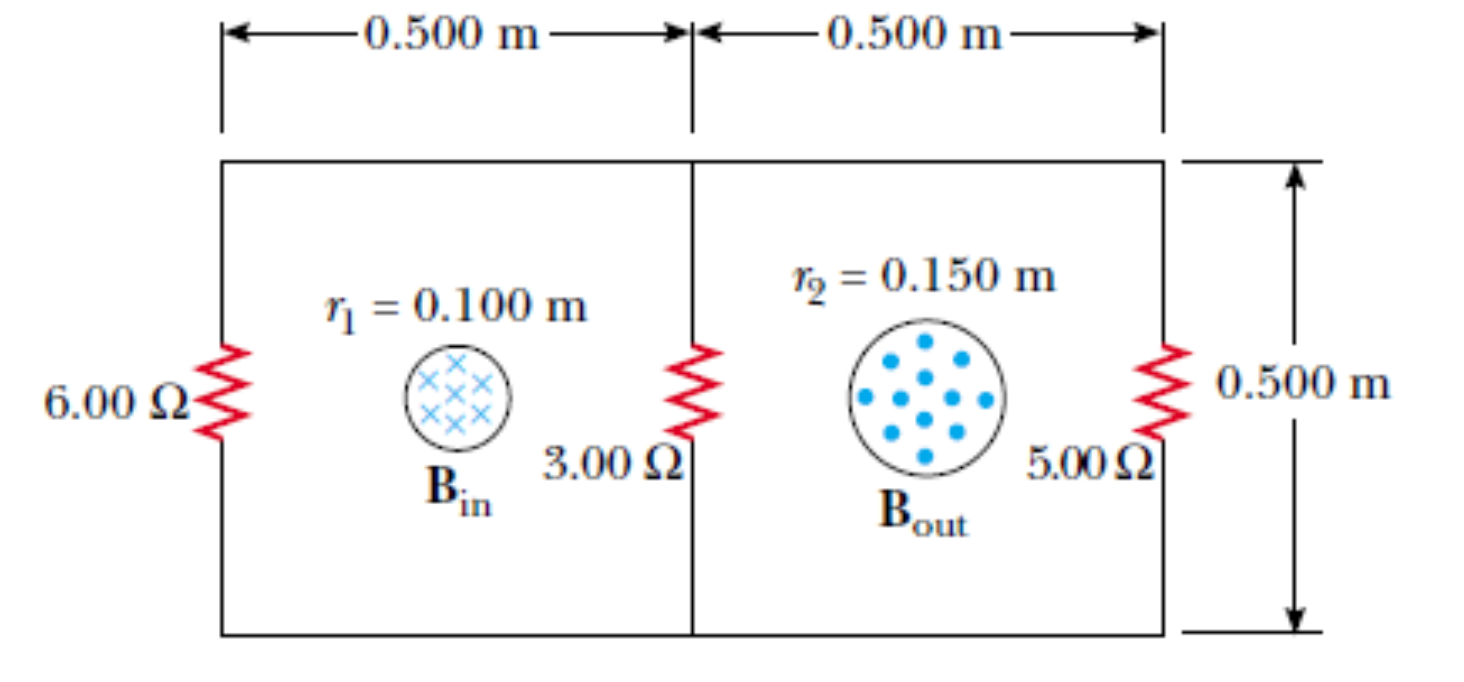
\includegraphics[scale = 0.3]{oz06/resources/Oz6Oef5.png}
    \end{center}

    \begin{description}[labelwidth=1.5cm, leftmargin=!]
        \item[Geg. :] $B_{\text{in}} = B_{\text{out}}$, $\frac{d}{dt} B_{\text{in}} = \frac{d}{dt} B_{\text{out}} = 100$ T/s, $R_1 = 6.0 \ \Omega$, $R_2 = 3.0 \ \Omega$, $R_3 = 5.0 \ \Omega$, $r_1 = 0.100$ m, $r_2 = 0.150$ m, $a = 0.500$ m
        \item[Gevr. :] $I_1$, $I_2$, $I_3$
        \item[Opl. :]
            In de linkse lus is de geïnduceerde emf gelijk aan
            \begin{equation*}
                \left| \mathcal{E}_{\text{ind}} \right| =  \frac{d\Phi_{B_{\text{in}}}}{dt} = A\frac{dB_{\text{in}}}{dt} = \pi r_1^2 \frac{dB_{\text{in}}}{dt}  = \pi \ \text{V}.
            \end{equation*}
            waarbij de stroom tegen-wijzerzin loopt, sinds $\frac{dB_{\text{in}}}{dt} > 0$. In de rechtse lus is de geïnduceerde emf gelijk aan
            \begin{equation*}
                \left| \mathcal{E}_{\text{ind}} \right| =  \frac{d\Phi_{B_{\text{in}}}}{dt} = A\frac{dB_{\text{in}}}{dt} = \pi r_2^2 \frac{dB_{\text{in}}}{dt}  = 2.25\pi \ \text{V}.
            \end{equation*}
            warbij de stroom wijzerzin loopt, sinds $\frac{dB_{\text{out}}}{dt} > 0$. We vinden met de wetten van Kirchhoff dat
            \begin{equation*}
                \begin{cases}
                    I_1 + I_2 = I_3 \\
                    6.00I_1 + 3.00I_2 - \pi = 0 \\
                    3.00I_2 + 5.00I_3 - 2.25\pi = 0 \\
                \end{cases}
            \end{equation*} 
            wat we kunnen oplossen tot:
            \begin{equation*}
                \begin{cases}
                    I_1 = 0.0622 \ \text{A} \\
                    I_2 = 0.923 \ \text{A} \\
                    I_3 = 0.860 \ \text{A} \\
                \end{cases}
            \end{equation*}
    \end{description}


\vspace{1cm}